\chapter{Feature Coverage Map}\label{app:feature_coverage_map}

Figure~\ref{fig:appd_coverage} provides a visual overview of all 59 agroclimatic features in the dataset, organised by variable family (rows) and phenological stage $\times$ window position (columns). Each coloured cell represents one or more feature windows: the darker upper half shows features computed for the current harvest year (y1); the lighter lower half shows features computed for the previous year (y0). The number inside each cell is the window width in days.

The map makes several structural properties of the feature set immediately visible. Flowering is the most densely populated stage, contributing features across all variable families and both years, reflecting the critical importance of flowering-phase conditions for yield determination. The previous-year (y0) features are concentrated at Flowering and Harvest, corresponding to the two biological carry-over mechanisms described in Section~\ref{sub:currentyear_vs_previousyear_features}: inflorescence primordia formation (driven by prior-year flowering thermal conditions) and vine carbohydrate reserve building (driven by prior-year harvest and post-harvest conditions). Bud Break and Start Maturity have sparser coverage --- only those specific variables with demonstrated agronomic relevance to those stages were included. The soil-water family (swa, stress days, saturation days) is notably concentrated at Flowering and Harvest, consistent with their role as the primary mechanistic pathways through which climate affects production identified in the CarenR rule analysis (Chapter~\ref{ch:goal_1_rule_extraction}).

\begin{landscape}
\begin{figure}[htbp]
  \centering
  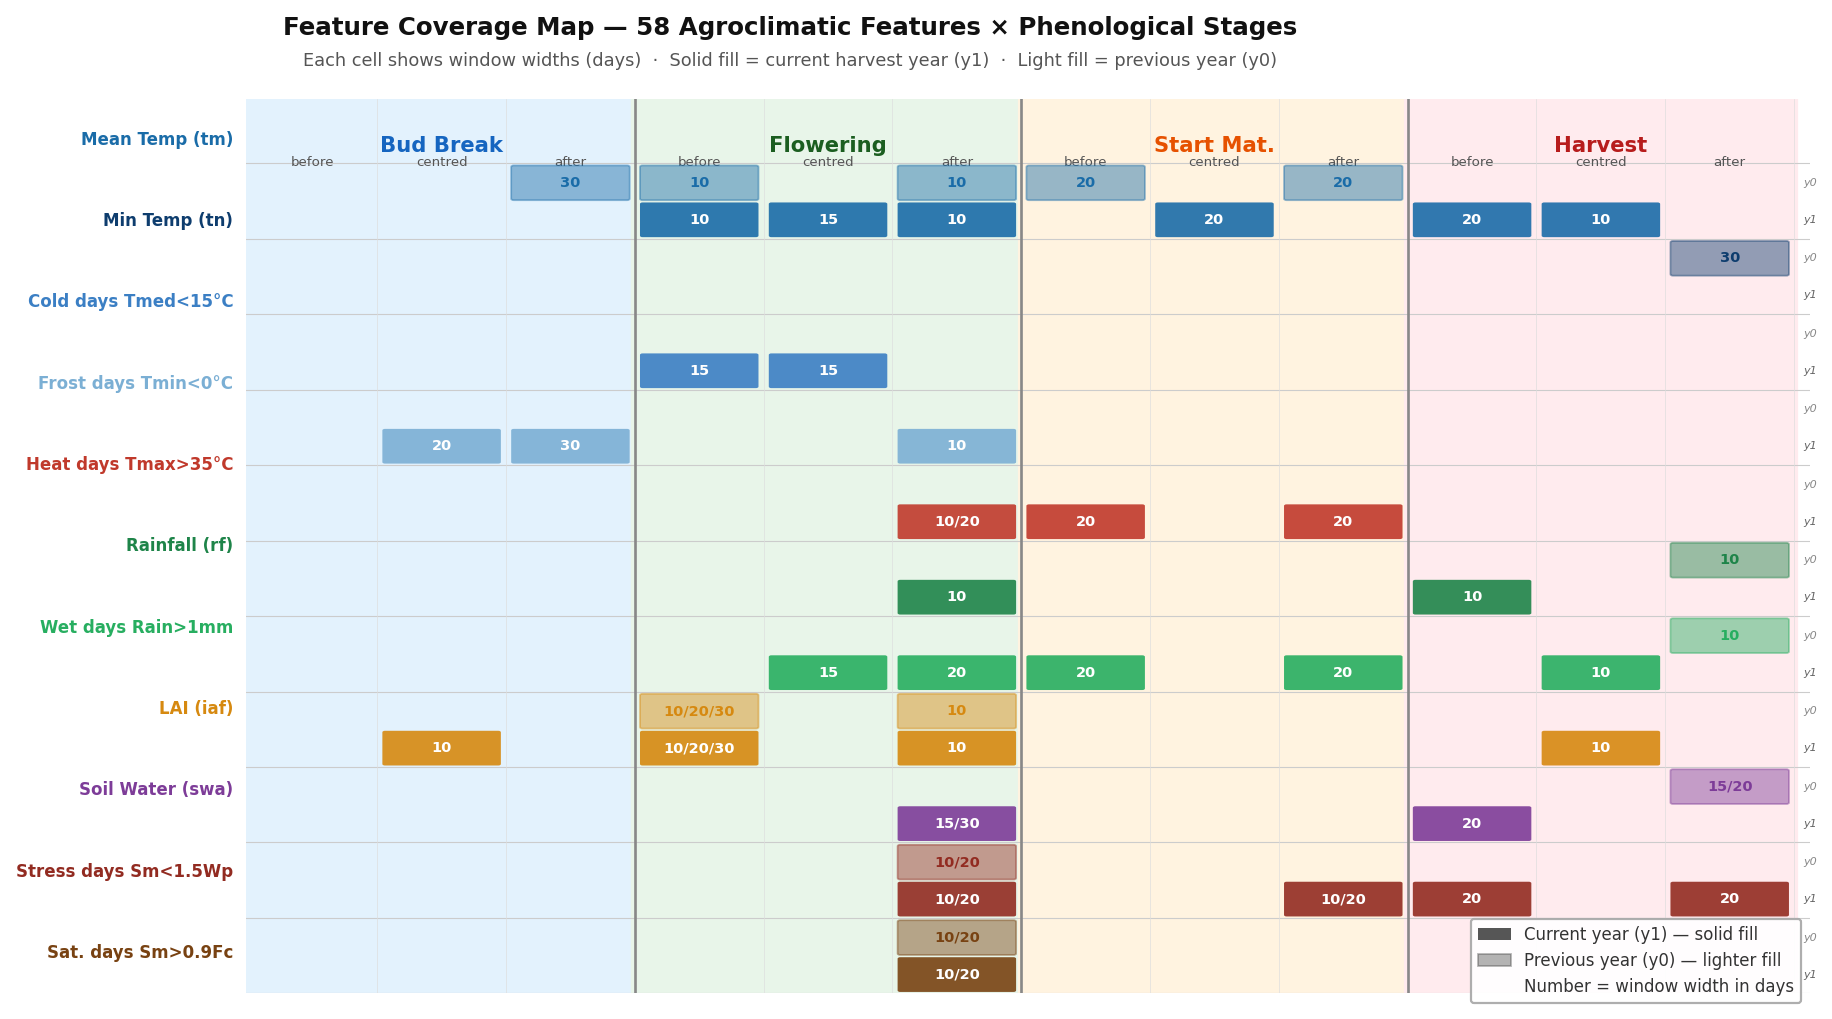
\includegraphics[width=\linewidth, height=0.85\textheight, keepaspectratio]{figures/fig_appd_1.png}
  \caption{Feature coverage map: 59 agroclimatic features by phenological stage and window position.}
  \label{fig:appd_coverage}
\end{figure}
\end{landscape}

\noindent Each coloured cell represents one or more feature windows. Darker shading (top half) = current year (y1); lighter shading (bottom half) = previous year (y0). Numbers inside cells indicate window width in days. Stage colour coding: \textcolor{blue}{blue} = Bud Break, \textcolor{green!60!black}{green} = Flowering, \textcolor{orange}{amber} = Start Maturity, \textcolor{red}{red} = Harvest.
